\begin{landscape}
\begin{figurels}[!]
    \caption{\fontsize{10pt}{12pt} Spectra gated on 123 keV ($2_{gs}^+\rightarrow 0_{gs}^+$) and 247 keV ($4_{gs}^+\rightarrow 2_{gs}^+$), the first two ground state band lines of $^{154}$Gd. As can be seen, some lines do not appear in different gates. Comparison of these gates, yields a list of transitions that directly populate the interim level (in this example, the $2^+$ state). Several peaks are circled in green that appear in the $2_{gs}^+\rightarrow 0_{gs}^+$ and not the $4_{gs}^+\rightarrow 2_{gs}^+$ transition.}
    \label{fig:154_GS_Gate}
\end{figurels}
\begin{figurels}[!]
    \centering
    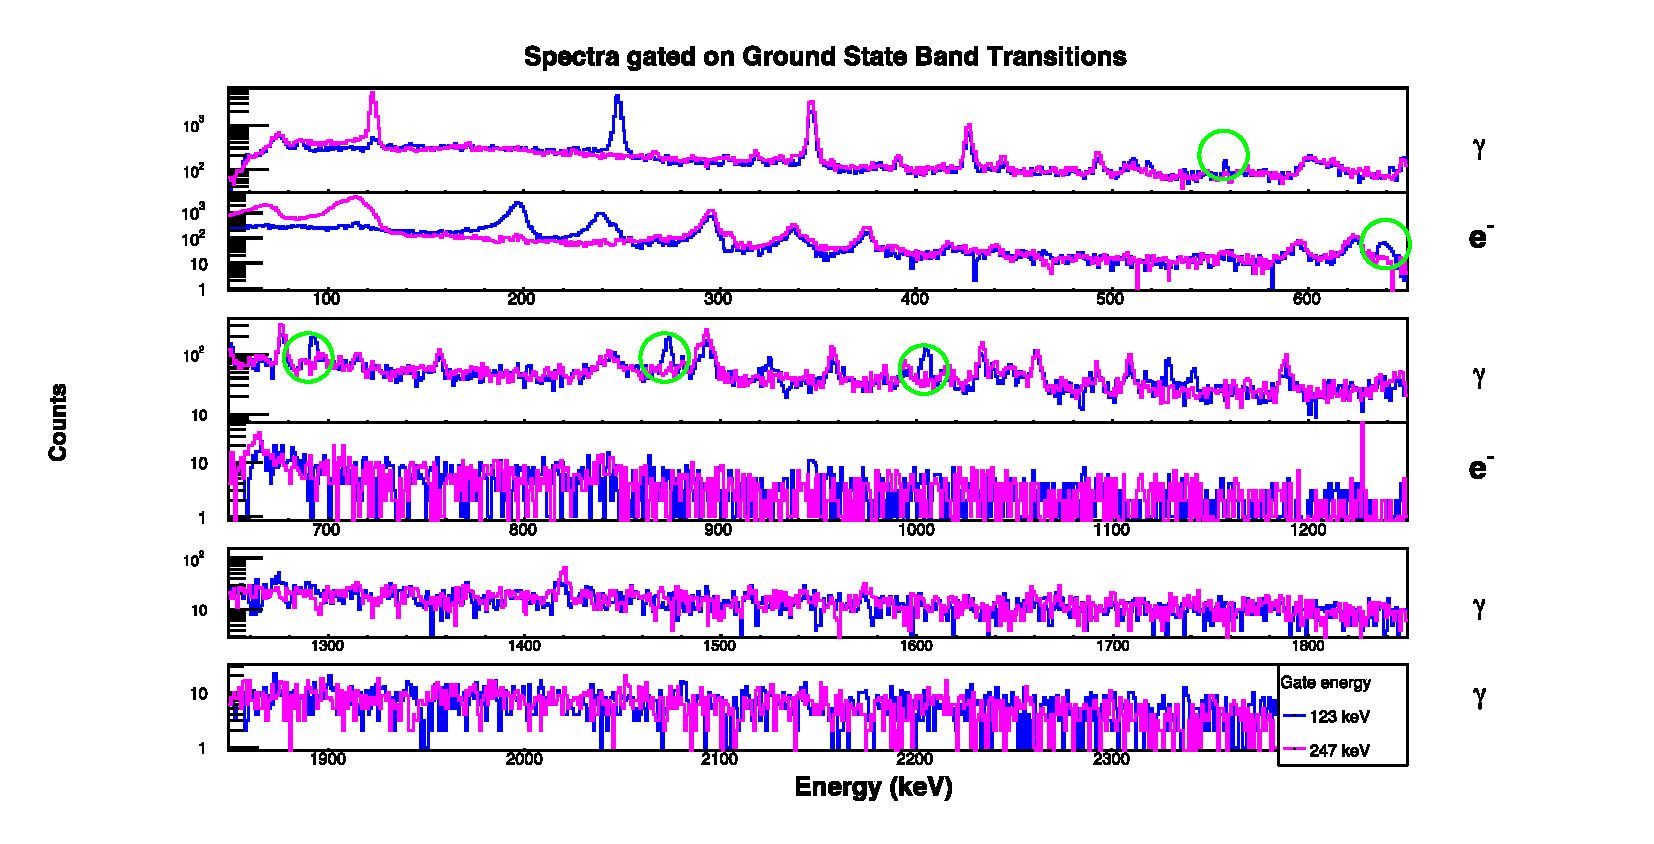
\includegraphics[scale=0.9]{154GdTablesAndFigs/154Gd_stacked.eps}
\end{figurels}
\end{landscape}